

\documentclass[letterpaper, 10 pt, conference]{ieeeconf}  % Comment this line out
                                                          % if you need a4paper
%\documentclass[a4paper, 10pt, conference]{ieeeconf}      % Use this line for a4
                                                          % paper

\IEEEoverridecommandlockouts                              % This command is only
                                                          % needed if you want to
                                                          % use the \thanks command
\overrideIEEEmargins
% See the \addtolength command later in the file to balance the column lengths
% on the last page of the document

\usepackage[utf8]{inputenc}
\usepackage[T1]{fontenc}
\usepackage{svg}


\usepackage{graphicx}
\usepackage{tabularx} % For adjustable column widths
\usepackage{ragged2e}
\usepackage{mdframed}
\usepackage{amsmath, amssymb}
\usepackage{algorithm}
\usepackage[noend]{algpseudocode}
\usepackage[caption=false,font=footnotesize]{subfig}
\usepackage{textcomp} % For \textprime (prime symbol) support
\usepackage{hyperref}
\usepackage[toc,page]{appendix}



\mdfdefinestyle{mybox}{%
    linewidth=1pt,
    frametitlerule=true,
    backgroundcolor=white,
    linecolor=black,
    innerleftmargin=10pt,
    innerrightmargin=10pt,
    innertopmargin=10pt,
    innerbottommargin=10pt
}

% The following packages can be found on http:\\www.ctan.org
%\usepackage{graphics} % for pdf, bitmapped graphics files
%\usepackage{epsfig} % for postscript graphics files
%\usepackage{mathptmx} % assumes new font selection scheme installed
%\usepackage{mathptmx} % assumes new font selection scheme installed
%\usepackage{amsmath} % assumes amsmath package installed
%\usepackage{amssymb}  % assumes amsmath package installed

\usepackage{tikz}
\usetikzlibrary{shapes.geometric, arrows.meta, positioning}
\usepackage[dvipsnames]{xcolor}

\usepackage{cite}

\title{\LARGE \bf
Machine Learning-Based Prediction of Uber and Lyft Prices Using Random Forest and Gradient Boosting}

%\author{ \parbox{3 in}{\centering Huibert Kwakernaak*
%         \thanks{*Use the $\backslash$thanks command to put information here}\\
%         Faculty of Electrical Engineering, Mathematics and Computer Science\\
%         University of Twente\\
%         7500 AE Enschede, The Netherlands\\
%         {\tt\small h.kwakernaak@autsubmit.com}}
%         \hspace*{ 0.5 in}
%         \parbox{3 in}{ \centering Pradeep Misra**
%         \thanks{**The footnote marks may be inserted manually}\\
%        Department of Electrical Engineering \\
%         Wright State University\\
%         Dayton, OH 45435, USA\\
%         {\tt\small pmisra@cs.wright.edu}}
%}



\author{Aditi Roy$^{1}$, Dulcie Archuleta$^{1}$, and Sachin Chandrasekara$^{1}$}


\begin{document}



\maketitle
\thispagestyle{empty}
\pagestyle{empty}


%%%%%%%%%%%%%%%%%%%%%%%%%%%%%%%%%%%%%%%%%%%%%%%%%%%%%%%%%%%%%%%%%%%%%%%%%%%%%%%%
\begin{abstract}

Accurate prediction of ride-hailing fares is a challenging problem due to the complex interaction between trip attributes and external factors such as weather. This study examines whether incorporating weather-related features improves the performance of machine learning models in predicting Uber and Lyft prices. The problem is formulated as a regression task using combined ride and weather datasets that include variables such as temperature, rainfall, wind, and pressure . Data preprocessing involved feature engineering, merging datasets based on time and location, handling missing values, and removing outliers using the interquartile range method. The dataset was then separated into Uber and Lyft subsets, and two models, Random Forest and Gradient Boosting, were trained and evaluated using RMSE and R$^$2 metrics. The results show that models trained without weather features produced higher prediction errors and lower accuracy, while the inclusion of weather information significantly improved model performance for both platforms. In particular, models achieved lower error values and higher goodness-of-fit after integrating environmental variables, with Random Forest consistently performing slightly better than Gradient Boosting. These findings indicate that weather conditions, especially rainfall, play an important role in influencing ride prices and that incorporating such features leads to more accurate and reliable prediction models for ride-hailing services.

\end{abstract}


%%%%%%%%%%%%%%%%%%%%%%%%%%%%%%%%%%%%%%%%%%%%%%%%%%%%%%%%%%%%%%%%%%%%%%%%%%%%%%%%
\section{Introduction}

Ride-hailing platforms such as Uber and Lyft have gained popularity in urban transportation systems largely due to convenience and affordability. These platforms have transformed modern transit by replacing traditionally used fixed-rate fare structures with dynamic pricing mechanisms \cite{d1}. These platforms utilize algorithmic "surge multipliers" to correct spatio-temporal imbalances between ride availability and rider demand in real-time \cite{d2}. Accurately predicting ride prices is critical to app functionality because it provides users with price transparency for departure planning, assists drivers in determining whether it is advantageous to relocate, and enables platforms to optimize vehicle allocation \cite{d3}.

Literature indicates that ride-hailing fares are determined by a multidimensional set of features such as trip distance and pickup and drop-off locations \cite{d1}. This creates a complex regression challenge where mixed numerical and categorical features interact in non-linear ways. This interaction makes supervised machine learning ensemble models like Random Forest and Gradient Boosting highly suitable for capturing generalizable patterns[4]. Because proprietary supply and demand data are often unavailable, predictive models rely on indirect environmental and ride-specific attributes \cite{d1}.

Time and weather conditions also influence transportation demand and fare fluctuations. For example, precipitation typically increases demand for taxi-like services while reducing the use of other modes of transportation \cite{d5}. Temperature exhibits complex, non-linear effects on ride-hailing activity, where demand often rises with temperature until \cite{d5,d3}. While previous studies have examined demand forecasting in major markets like New York and Chicago, there is a demand for clearer trip-level price prediction in other major metropolitan areas. Merging ride-hailing records with local hourly weather observations allows for a nuanced understanding of how environmental factors impact local pricing \cite{d7, d4}.

The objective of this project is to develop and evaluate separate machine learning regression models for Uber and Lyft trip prices in Boston. By integrating distance, location features, weather variables (temperature, rain, wind, and pressure), and a categorical time-of-day feature, the project aims to accurately estimate ride fares and provide insights into platform-specific pricing variations.

\begin{figure*}[htbp]
\centering
\begin{mdframed}[linecolor=black, linewidth=0.5pt, roundcorner=5pt]
    \centering
    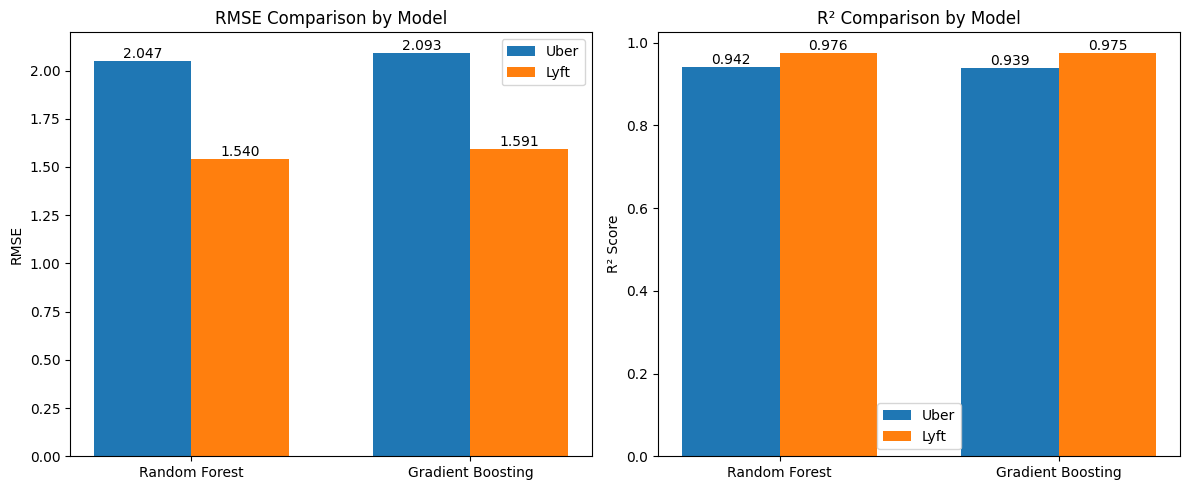
\includegraphics[width=1\textwidth]{Images/output_1.png}

\end{mdframed}

  \caption{Comparison of RMSE and $R^2$ scores for Random Forest and Gradient Boosting models without weather features}
    \label{cv}
\end{figure*}


\section{Materials and Methods}

\subsection{Dataset}

The dataset used in this study provides information about uber-lyft cab ride services, including distance, time, and other ride-related factors. The purpose of this project is to predict the cost of a cab ride using these input features. The original dataset contains 693,071 rows and 10 columns. Each row represents a single cab ride, and the columns indicate various aspects of the ride. And other dataset is weather which includes weather information such as temperature, rain, humidity, wind, and pressure.


\subsection{Data Preprocessing}

Data preprocessing was used to prepare the dataset for model training and to increase the overall stability of the models. Initially, a legible date-time format was created from the time data in both datasets. The location, date, and hour were then combined to create a new feature. This made it easier to connect the weather data with the taxi data. The weather data was then grouped by time and location, and the mean values were computed. The rain variable's missing values were substituted with zero. Based on the shared location and time feature, the two datasets were then combined into a single dataset. In order to ensure clean data, rows with missing values were eliminated.

The Interquartile Range (IQR) approach was used to find outliers in the price column. To enhance model performance, values outside the permitted range were eliminated. Based on the type of taxi, the dataset was split into two groups: Uber and Lyft. Every group was examined independently. The goal variable (price) and characteristics (X) were kept apart for both datasets. The data was then divided into training (80\%) and testing (20\%) sets.

\subsection{Method}


\subsubsection{Random Forest Regressor (RFR)}
A machine learning model called Random Forest Regressor (RFR) makes predictions by utilizing a large number of decision trees. A random sampling of the data is used to construct each tree, and the average of the outcomes from each tree is used to get the final forecast. This improves accuracy and lowers errors. In order to capture complex correlations between characteristics and taxi prices, Random Forest was employed in this project. It can handle non-linear patterns with minimal preprocessing and performs well with both numerical and categorical data \cite{s1}.


\subsubsection{Gradient Boosting Regressor}

Gradient Boosting Regressor is an ensemble technique that gradually constructs numerous tiny decision trees \cite{s2}. This technique is effective at identifying intricate relationships and typically provides accurate predictions for structured data. 


\section{Results}

Table \ref{tab:no_weather} and Figure \ref{cv} showed the performance of the models without weather features. When weather information was not included, the models had lower accuracy and higher RMSE values. 


\begin{table}[ht]
\centering
\caption{Model performance without weather features}
\label{tab:no_weather}
\begin{tabular}{llccc}
\hline
\textbf{Cab Type} & \textbf{Model} & \textbf{MSE} & \textbf{RMSE} & \textbf{$R^2$} \\
\hline
Lyft & Random Forest & 13.08 & 3.62 & 0.870 \\
Uber & Random Forest & 5.54 & 2.35 & 0.923 \\
Lyft & Gradient Boosting & 13.98 & 3.74 & 0.861 \\
Uber & Gradient Boosting & 6.43 & 2.53 & 0.911 \\
\hline
\end{tabular}
\end{table}


\begin{figure*}[htbp]
\centering
\begin{mdframed}[linecolor=black, linewidth=0.5pt, roundcorner=5pt]
    \centering
    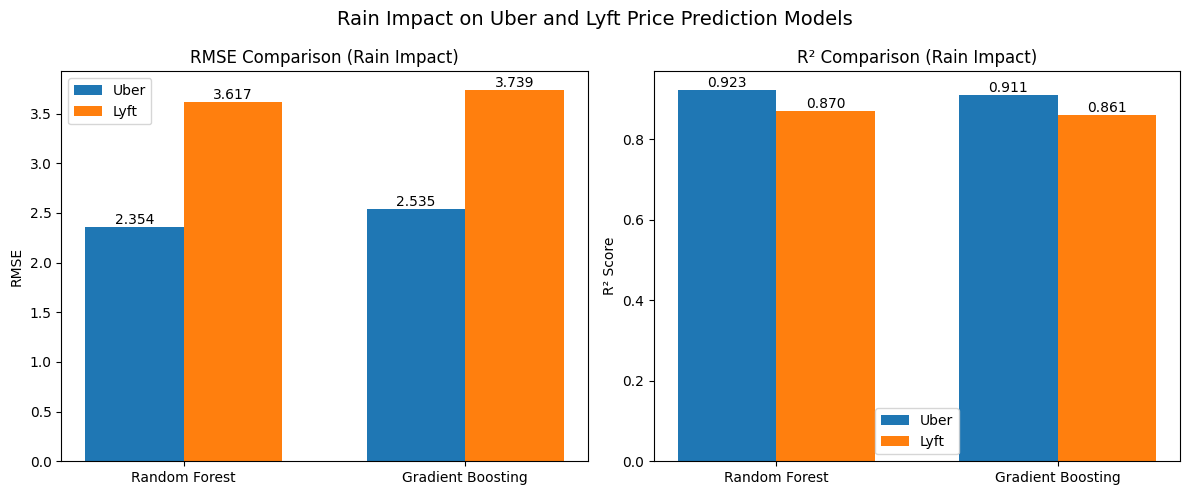
\includegraphics[width=1\textwidth]{Images/output_2.png}

\end{mdframed}

\caption{Impact of weather (rain) on RMSE and $R^2$ scores for Uber and Lyft price prediction models}
    \label{f2}
\end{figure*}

\begin{table}[ht]
\centering
\caption{Model performance with weather features}
\label{tab:with_weather}
\begin{tabular}{llccc}
\hline
\textbf{Cab Type} & \textbf{Model} & \textbf{MSE} & \textbf{RMSE} & \textbf{$R^2$} \\
\hline
Lyft & Random Forest & 2.37 & 1.54 & 0.976 \\
Uber & Random Forest & 4.19 & 2.05 & 0.942 \\
Lyft & Gradient Boosting & 2.53 & 1.59 & 0.975 \\
Uber & Gradient Boosting & 4.38 & 2.09 & 0.939 \\
\hline
\end{tabular}
\end{table}


Also Table \ref{tab:with_weather} and Figure \ref{f2} shows the performance of the models with weather features. After adding weather information, both the Uber and Lyft datasets performed considerably better. 

\section{Data and Code Availability}

The scripts and summary outputs supporting this study are available in a public GitHub repository \url{https://github.com/sachinkavindaa/ML_uber_lyft_project}. 

\section{Conclusion}

Machine learning algorithms have been used in this work to predict Uber and Lyft fares based on ride data and weather information. The Random Forest and Gradient Boosting models were evaluated and compared. The findings suggest that both models did a good job of predicting prices. But in most cases, Random Forest outperformed Gradient Boosting by a small margin. A key finding of this study is the importance of weather data. When weather features were included, the model performance improved significantly. This demonstrates that variables like rainfall and temperature have a significant impact on taxi fares and should not be neglected. Overall, this study demonstrates how price prediction models can be enhanced by integrating ride data with meteorological data. Building more effective pricing systems and understanding how various factors impact taxi fares can both benefit from these findings.



























 
\begin{thebibliography}{99}


\bibitem{d1} M. Battifarano and Z. Qian, “Predicting real-time surge pricing of ride-sourcing companies,” Transportation Research Part C: Emerging Technologies, vol. 107, pp. 444–462, 2019, doi: 10.1016/j.trc.2019.08.019.

\bibitem{d2} S. Jiang, L. Chen, A. Mislove, and C. Wilson, “On ridesharing competition and accessibility: Evidence from Uber, Lyft, and taxi,” in Proc. 2018 World Wide Web Conf. (WWW), Lyon, France, 2018, pp. 863–872, doi: 10.1145/3178876.3186134.

\bibitem{d3}L. Chen, P. Thakuriah, and K. Ampountolas, “Short-term prediction of demand for ride-hailing services: A deep learning approach,” J. Big Data Anal. Transp., vol. 3, pp. 175–195, 2021, doi: 10.1007/s42421-021-00041-4.


\bibitem{d4} M. Taiebat, E. Amini, and M. Xu, “Sharing behavior in ride-hailing trips: A machine learning inference approach,” Transportation Research Part D: Transport and Environment, vol. 103, Art. no. 103166, 2022, doi: 10.1016/j.trd.2021.103166.

\bibitem{d5} S. Lepage and C. Morency, “Impact of weather, activities, and service disruptions on transportation demand,” Transportation Research Record, vol. 2675, no. 1, pp. 294–304, 2021, doi: 10.1177/0361198120966326.

\bibitem{d6} A. A. Williams, J. G. Allen, P. J. Catalano, J. J. Buonocore, and J. D. Spengler, “The influence of heat on daily police, medical, and fire dispatches in Boston, Massachusetts: Relative risk and time-series analyses,” Am. J. Public Health, vol. 110, no. 5, pp. 662–668, May 2020, doi: 10.2105/AJPH.2019.305563.

\bibitem{d7} K. Sundravadivelu, G. E. Rani, K. Karthigadevi, M. Thenmozhi, M. Sakthimohan, and V. S. Kumar, “Taxi fare prediction using random forest: A data-driven approach based on pickup/dropoff locations and ride attributes,” unpublished.

\bibitem{s1} L. Breiman, “Random forests,” Machine Learning, vol. 45, no. 1, pp. 5–32, 2001..

\bibitem{s2} J. H. Friedman, “Greedy function approximation: A gradient boosting machine,” Annals of Statistics, vol. 29, no. 5, pp. 1189–1232, 2001.






\end{thebibliography}




\end{document}
